\documentclass[12pt, onecolumn]{article}
\usepackage{graphicx}
\usepackage{appendix}
\usepackage{placeins}
\usepackage{siunitx}
\usepackage{amsmath}
\usepackage{caption}
\usepackage{subcaption}
\usepackage{adjustbox}
\usepackage[margin=1in]{geometry}
\usepackage{pgfplotstable}
\usepackage{pgfplots}
\usepackage{multirow}
\usepackage{graphicx}
\usepackage{placeins}
\usepackage{longtable}
\usepackage{color, hyperref} 
\usepackage{float}
\usepackage{tikz}
\usepackage{placeins}
\usepackage{listings}
\newcommand\tab[1][1cm]{\hspace*{#1}}
\usepackage[style=ieee, sorting=none]{biblatex}
\addbibresource{ref.bib}
\pagestyle{plain}
\begin{document}

\begin{titlepage}
\begin{center}   


\vspace{3 cm}


\rule{500pt}{1pt}\\
\vspace{0.5cm}
\textbf{\LARGE Design of an Adaptive Hearing Aid}
\rule{500pt}{1pt}\\
\vspace{1cm}
\textit{Daniel Edwards - 1055301 \\ 23/10/2018}



\begin{figure}[h]
\centering

\includegraphics[width=4cm]{schoolLogo.png}
\end{figure}
\textit{School of Electrical \& Information Engineering, University of the
Witwatersrand, Private Bag 3, 2050, Johannesburg, South Africa}

\end{center}
\section*{Abstract}

This is my abstract
\end{titlepage}

\tableofcontents
\newpage

\section{Introduction}

define what adaptive means

\section{Background}

\noindent Hearing loss is a common problem in society. In \textit{2016}, the University of the Witwatersrand released a statement saying that in South Africa, approximately $20\%$ of the population suffers from a form of hearing loss \cite{witsHearingStats}. As a result of hearing loss, an individual can suffer from loneliness, isolation, dependence, depression and frustration. These are signs of poor quality of \cite{qualityOfLife}. The amount of people with an impaired quality of life provides motivation for the necessity of devices to improve an individuals hearing namely; a hearing aid. 


\section{Design Research}

****Talk about conductive hearing loss

\noindent Many factors contribute to hearing loss. A common type is conductive hearing loss \cite{earinfo}. This is a result of age, excessive noise or various diseases \cite{hearIt}. This is a permanent form of hearing loss which can be treated with hearing assisting devices \cite{hearIt}. This section presents an analysis of existing solutions to this problem and a literature review.

\subsection{Existing Solutions}

\noindent Two main hearing assisting devices exist for sensorineural hearing impairments namely; hearing aids and cochlear implants \cite{atlantic}. Cochlear implants are typically used in cases of extreme sensorineural hearing loss. These devices work well in quiet environments \cite{carroll}. However, cochlear implant users battle to perceive speech in noisy environments \cite{carroll} and thus, the individuals quality of life is not improved. Therefore, this design will make use of hearing aid technology.\\
\newline
\noindent There are two main types of hearing aids, analogue and digital. Analogue hearing aids amplify all sounds, which includes the important sound and noise which is not ideal \cite{woodford}. Ricketts \cite{ricketts} states that the largest problem for the hearing impaired is listening in noisy situations. Digital hearing aids however, contain a signal processing element which gives them additional functionality such as filtering noise and isolating sounds in specific directions \cite{ricketts}. \\

put something in about Ricketts and avoiding noise - isolation, say something about adaptive

\subsection{Literature Review}
\label{sec:litReview}

\noindent Sebastian \textit{et al.} \cite{sebastian} defines a hearing aid, as an electro-acoustic device with the purpose of making speech intelligible. This purpose, together with the patients quality of life, must be at the center of each design decision.\\
\newline
\noindent Audiograms, performed by audiologiests, are used to detect hearing impairments on a patient \cite{audiogram}. An audiogram illustrates the hearing threshold of a person at different pitches and frequencies \cite{sebastian}. These graphs illustrate the frequencies at which the patient battles to hear. Frequency response matching is a technique utilised by hearing aids to correct the audiogram of the patient. Kakol \textit{et al.} mention that in many cases, patients experience hearing difficulties at different frequency ranges \cite{diffMeth}. Therefore, by correcting the audiogram at the required frequencies, the patients hearing can be improved. This correction can be implemented with a series of filters which apply gain to various frequency bands \cite{diffMeth}. This method is also mentioned by Sebastian \textit{et al.} and is referred to as selective amplification \cite{sebastian}.\\
\newline
\noindent Sebastian \textit{et al.} provide an frequency response matching (FRM) investigation between uniform and non-uniform filter banks \cite{sebastian}. The frequency bands in uniform filter banks are equally spaced whereas non-uniform filter banks are arbitrary. Non-uniform filter banks are the preferred choice as they allow for an audiogram to be correct at the precise frequency bands that are affected by hearing loss \cite{sebastian}. According to Sebastian \textit{et al.}, the frequency bands at the critical hearing frequencies should be narrow for the best compensation \cite{sebastian}. Therefore, this design will consider narrow frequency band, non-uniform filter banks for audiogram correction. \\
\newline
\noindent Chang \textit{et al.} give further insight into the types of filter banks by providing four different types namely; uniform, critical-like, symmetric and $1/3$ octave \cite{chang}. The $1/3$ octave filter bank proved to have the best audiogram matching. However, it had a $78ms$ delay at $24kHz$ compare to a $27ms$ delay when parallel \textit{IIR} filters were used. Shearman \cite{octave} states a better understanding of how people perceive sound can be achieved by using octave analysis as breaking signals in octaves allows for the quality of the signal to be measured. This design aims to optimise the sound quality to improve the patients quality of life and thus, octave analysis must be considered.\\
\newline 
\noindent Dhawan \textit{et al.} simulate filtering in a hearing aid while using a wavelet filter to reduce noise. Additive white Gaussian noise (AWGN) was used to simulate the auditory noise \cite{dhawan}. Noise reduction is a critical component of this design and thus, the effect of these noise reduction techniques will be investigated within this system. \\
\newline
\noindent Ricketts \cite{ricketts} provides hearing aid performance metrics to raise the hearing capability of a hearing impaired individual to that of a normal hearing person. Normal hearing people, require an \textit{SNR\footnote{Signal to noise ratio.}} of at least $+6dB.$ as suggested by \cite{moore}. Hearing impaired individuals however, require an \textit{SNR} greater than $+6dB$ to achieve sufficient hearing \cite{tillman}. This increase \textit{SNR} requirement is because impaired hearing caused by poor hearing thresholds, results in noise related problems \cite{ricketts}. For children, a \textit{SNR} of $+15dB \rightarrow +30dB$ is required for educational purposes. Ricketts also stated that by tuning the hearing aid to listen in the direction of the source can improve the \textit{SNR} by about $3dB \rightarrow 6dB$.\\
\newline
\noindent Chen \textit{et al.} \cite{present} suggest that using multiple microphones results in better extraction, separation of frequencies and localization of the source whilst reducing noise, interference, echo and reverberation. This provides motivation for utilising a multiple microphone array in this design. Resource \cite{broadEnd} provides a comparison between two microphone array designs namely; broadside and endfire. This paper shows that the broadside configuration attenuates the signal less at low frequencies and has a larger bandwidth compared to the endfire configuration. The endfire configuration however, had better directivity when placed in the desired sound direction \cite{broadEnd}. In addition, McCowan \cite{mccowan} states that voice is a broadband signal. Therefore, in terms of array configuration, a trade-off must be made between bandwidth and directivity performance.  \\
\newline
\noindent Munir \cite{munir} states that in telephony systems, a frequency range of $300Hz$ to $3.4kHz$ is used because this is the frequency range of voice. The human ear however, can detect a frequency range of $20Hz$ to $20kHz$. Audiograms however, typically test upto a maximum frequency of $8kHz$ \cite{audioMaxFreq}. Since this system aims to correct audiograms, this frequency range must be considered.\\
\newline
\noindent McCowan \cite{mccowan} provides a comprehensive explanation of the wave propagation and various algorithms to determine directivity. This paper evaluates the performance of these algorithms within this context to determine the optimum solution.

Put something in about the number of bands that increases the matching error
Put the stuff about the audiogram gain factor thingy\\
mention stuff about why digital is better than analog\\
talk about group delay
\section{Design Objectives}

\noindent What the design intends to solve.

\section{Design Requirements}


\section{Design Assumptions and Constrains}

\subsection{Assumptions}

\noindent This paper presents a theoretical design and hence, assumptions can be made. This design is not limited by cost, power or space requirements. This design is considered for adult hearing only. The directionality component considers a $2D$ wave in a plane instead of a $3D$ wave. Finally, it is assumed that the speaker is deep inside the ear and hence separated from the microphone significantly enough such that feedback cancellation is not required.

\subsection{Constraints}

\noindent This system is constrained to a bandwidth of $20Hz$ to $8kHz$ to correspond to the audiogram frequency range.

constrains: 8kHz, response time

\section{Design Methodology}

\noindent The design of this system consists of two main subsystems. The first is the audiogram correction using an adaptive filter bank. The second, is applying directionality techniques to the signal to allow for the user to listen in specific directions. These subsystems will be amalgamated into a single system. This paper focuses on the adaptive hearing subsystem.\\
\newline
\noindent In this system, the adaptive filtering component is optimised for the audiogram matching error and response time. 


Mention the compression aspect\\
compare a bunch of different designs\\
find the best one\\
choose DSP and stuff from there\\
digital filters\\
ideal filter bank

\section{Adaptive Filter Design}

State the factors that contribute to the optimisation\\
\noindent The adaptive filter is a filter bank which consists of an array of bandpass filters. Each of the bandpass filters operate with a particular frequency range and gain. This design subsection aims to utilise this frequency bank rectify a patients audiogram. This audiogram is presented in Section \ref{sec:audiogram}.\\

\noindent \textbf{Approach:} Research proved that there are multiple filter bank types used to rectifying a patients audiogram. To determine the optimum design, each of these systems will be considered. Sections \ref{sec:uniDesign}, \ref{sec:critDesign}, \ref{sec:symmDesign} and \ref{sec:octDesign} present the design of the uniform, critical-like, symmetric and $1/3$ octave filter banks with similar design consideration discussed in Section \ref{sec:numFreqBands}...XXX. These designs will also be compared to the ANSIXXX specification presented in Section \ref{sec:ansi}.

Mention stuff about uniform and non-uniform filter banks

\subsection{Audiogram}
\label{sec:audiogram}

\noindent The audiogram considered in this design corresponds to a patient with conductive hearing loss. Audiologists measure a patients hearing typically at $125Hz$, $250Hz$, $500Hz$, $1kHz$, $2kHz$, $4kHz$ and $8kHz$ REF. MATLAB's \texttt{pchip} function was used to interpolate these values to provide hearing threshold values for the full $125Hz$ to $8kHz$ range. Reference \cite{mahmoud} provides audiograms for normal hearing and conductive hearing loss. Figure \ref{fig:normCondAudio} illustrates these audiograms.

\begin{figure}[h]
\centering
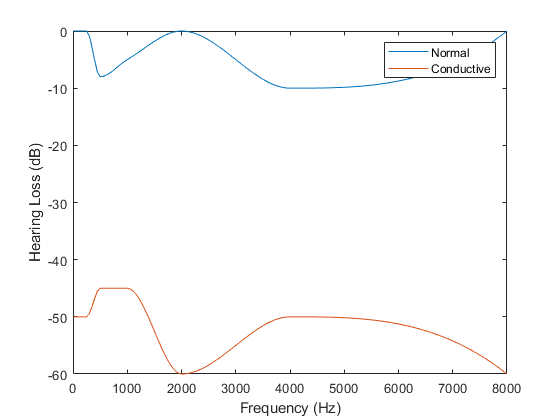
\includegraphics[width=0.6\linewidth]{normCondAudiogram.PNG}
\caption{Audiogram for Normal Hearing and Conductive Hearing Loss}
\label{fig:normCondAudio}
\end{figure}  

\noindent The filter bank aims match the conductive hearing loss patients audiogram to the normal hearing audiogram.

\subsection{Insertion Gain}
\label{sec:insertGain}

\noindent The filter bank corrects the audiogram by applying gain to particular frequencies. This is defined as insertion gain. In this design, the insertion gain is calculated using the NAL-R formulas given in equation \ref{eqn:nalRp}.

\begin{equation}
\label{eqn:nalRp}
\begin{aligned}
H_{3FA} &= (H_{500} + H_{1k} + H_{2k})/3 \\
X &= 0.15 \times H_{3FA} \\ 
IG_i &= X + (0.31\times H_i) + k_i
\end{aligned}
\end{equation}

\noindent Where X is XXXXXX, $IG_i$ is the insertion gain, $H_i$ is the audiogram value at the $i^{th}$ sampled frequency and $k_i$ is a constant at the $i^{th}$ sampled frequency given by Table \ref{tab:kiVal} in Appendix \ref{app:insertGainParam}. Similarly to the audiogram, the insertion gain values were interpolated using \texttt{MATLAB's} \texttt{pchip} function. The insertion gains for the full frequency range is illustrated in Figure \ref{fig:igFreqRange}.

\begin{figure}[h]
\centering
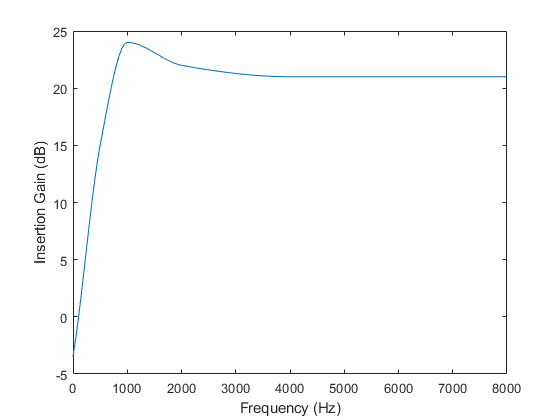
\includegraphics[width=0.6\linewidth]{igFreqRange.PNG}
\caption{Interpolated Insertion Gain for Full Frequency Range}
\label{fig:igFreqRange}
\end{figure}  

\subsection{Number of Filters} 
\label{sec:numFreqBands}

\noindent As stated above, the filter bank consists of multiple bandpass filters, each with a specific sub-band. Therefore, the number of filters used must be investigated, particularly for the uniform, critical-like, symmetric and $1/3$ octave filter banks designs. A uniform filter bank was used to investigate the effect that increasing the number of filters has on matching error and computational complexity. Appendix \ref{app:numFilt} provides the details of the filters used in this investigation. Figure \ref{fig:numBandsErrorFreq} and \ref{fig:numBandsErrorBand} illustrate the matching error for each band across the frequency range and the mean error for each number of frequency bands respectively.

\begin{figure}
\centering
\begin{minipage}{.45\linewidth}
  \centering
  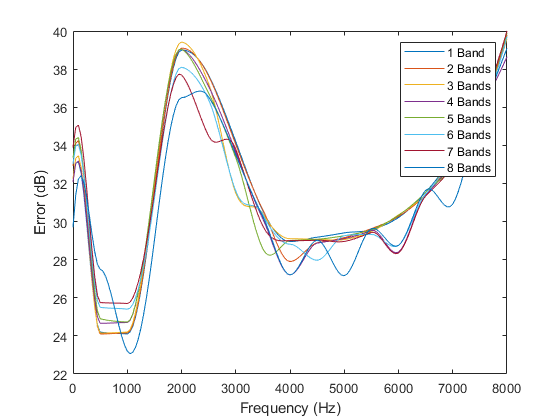
\includegraphics[width=0.9\linewidth]{numBandsErrorFreq.png}
  \captionof{figure}{Matching Error Across Frequency Spectrum per Filter Bank}
  \label{fig:numBandsErrorFreq}
\end{minipage}%
\begin{minipage}{.45\linewidth}
  \centering
  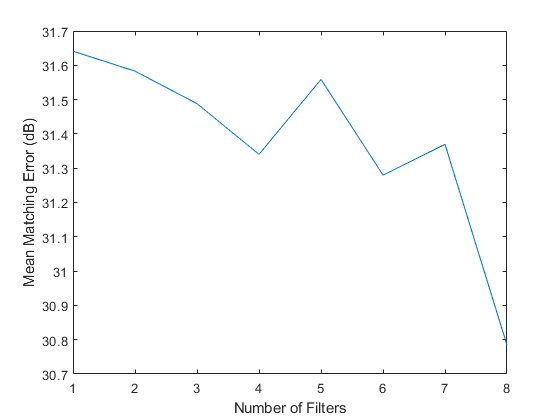
\includegraphics[width=0.9\linewidth]{numBandErrorBand.png}
  \captionof{figure}{Mean Matching Error per Filter Bank}
  \label{fig:numBandsErrorBand}
\end{minipage}
\end{figure}

\noindent This section investigates the effect of increases the number of filters in the filter bank. The large errors therefore, are not a concern at this point. Figure \ref{fig:numBandsErrorBand} illustrates that increasing the number of bands, decreases the mean matching error. Therefore, the design should aim to maximise the number of filters.

the number of filters emphasises the frequency bands that need to be adjusted.

\section{Uniform, Critical-like, Symmetric and Octave Filter Bank Design}

\noindent This section aims to optimise the structure of the filter bank's frequency bands. Therefore, a comparison between a uniform (Section \ref{sec:uniDesign}), critical-like (Section \ref{sec:critDesign}), symmetric (Section \ref{sec:symmDesign}) and octave (Section \ref{sec:octDesign}) filter banks will be made. The best performing filter bank will then be compared to the ANSIXXX designed in Section \ref{sec:ansi}. To draw a fair comparison, all of the filters will be design with the parameters given in Table \ref{tab:numFilt_FiltSpec} in Appendix \ref{app:numFilt}. Each filter bank will consist of $8$ bandpass filters. Furthermore, since a comparison is being drawn, the same insertion gain method as in Section \ref{sec:insertGain} will be used.

\subsection{Uniform Filter Bank Design}
\label{sec:uniDesign}

\noindent A uniform filter bank consist of an array of evenly spaced, filters with equal bandwidths \cite{chang}. Uniform filter banks are simple and easy to implement. However, for a sufficient resolution, uniform filter banks requires more bands than non-uniform filter banks for a good fit. The additional filters implies that more computations are required and thus, the filter bank's group delay is potentially increased \cite{brennan}. Section \ref{sec:numFreqBands}'s simulation utilised a uniform filter bank which yielded a mean matching error of $30.78dB$.


\subsection{Critical-like Filter Bank Design}
\label{sec:critDesign}

\noindent This filter is forms part of the non-uniform filter bank category. This filter design attempts to account for the psychoacoustic characteristics using the critical bands of the Bark Scale \cite{chong}. Table \ref{tab:bark} in Appendix \ref{app:bark} provides the Bark scale's critical frequency band information. In this investigation, we are limited to using $8$ filters and a maximum frequency of $8kHz$. Therefore, the filters will correspond to the frequency bands in Table \ref{tab:critFiltFreqBand} of Appendix \ref{app:critFiltFreqBand}.	This design achieved an average and maximum matching error of $0.8957dB$ and $11.4dB$ respectively. The matching error for the full frequency spectrum is illustrated in Figure \ref{fig:critMatErr}.


\begin{figure}[h]
\centering
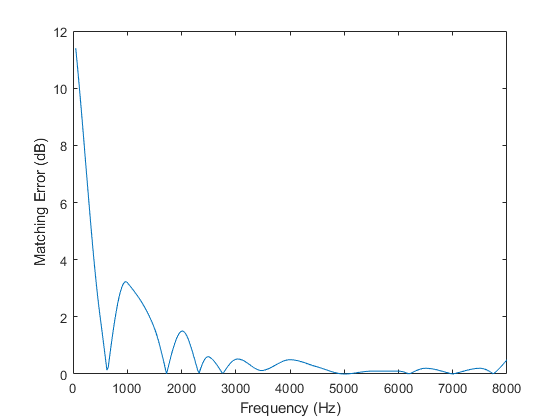
\includegraphics[width=0.6\linewidth]{critMatErr.PNG}
\caption{Matching Error for Critical-Like Filter Bank}
\label{fig:critMatErr}
\end{figure}  


\subsection{Symmetric Filter Bank Design}
\label{sec:symmDesign}

\noindent Symmetric filter banks provde an improvement on the uniform filter bank. The non-uniform sub-bands are symmetric about the center frequency of the frequency spectrum, in this case $4kHz$. Symmetric filter banks have the ability of enhancing the matching error of low and high, or mid frequencies \cite{sebastian}. Figure \ref{fig:normCondAudio} illustrates that the threshold of a conductive hearing loss patient is worse at the low and high frequencies. Therefore, the frequency bands will be chosen such that these frequencies are emphasised. Table \ref{tab:symFreqBand} in Appendix \ref{app:symFreqBands} illustrates the bands used in this investigation. Simulation illustrated that the symmetric filter bank acheived an average error of $0.795dB$ with a maximum matching error of $6.44dB$.  The matching error for the full frequency spectrum is illustrated in Figure \ref{fig:symMatErr}.

\begin{figure}[h]
\centering
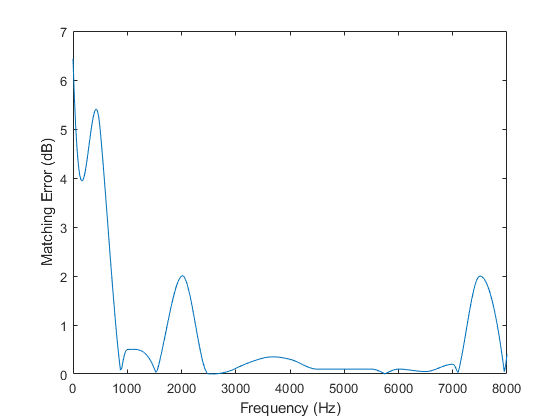
\includegraphics[width=0.6\linewidth]{symMatErr.PNG}
\caption{Matching Error for Symmetric Filter Bank}
\label{fig:symMatErr}
\end{figure}  



\subsection{Octave Filter Bank Design}
\label{sec:octDesign}

\noindent As stated above, separating a frequency spectrum into octaves allows for the quality of sound to be measure and by derivative, improved \cite{octave}. It is therefore natural for a filter bank to be designed using this principle. Each filter bank sub-band will have a center frequency relative to the reference sub-band center frequency $f_c [0] = 1000Hz$ \cite{octFreqCalc}. The center frequency of each sub-band is calculated using equation \ref{eqn:octCentFreq}. The corresponding upper $(f_{cu})$ and lower $(f_{cl})$ passband frequencies are calculated using equation \ref{eqn:octFreqEdge} \cite{octFreqCalc}.
%
\begin{equation}
\label{eqn:octCentFreq}
f_c[k-1] = f[k]/2 
\end{equation}
\begin{equation}
\begin{aligned}
\label{eqn:octFreqEdge}
f_{cu}[k] &= \frac{f_c[k] }{2^{1/2}}\\
f_{cl}[k] &= 2^{1/2}\times f_c[k]
\end{aligned}
\end{equation}
%

\noindent The center frequencies for this filter bank are chosen to be $63Hz$, $125Hz$, $250Hz$, $500Hz$, $1kHz$, $2kHz$, $4kHz$ and $8kHz$ which results in the filter specifications given in Table \ref{tab:octFreqBands} of Appendix \ref{app:octFreqBands}.

\section{ANSIXXXX Design}
\label{sec:ansi}

\section{Dynamic Compression Design}

\section{Success Criterion}


\section{Critical Evaluation of Results}



\subsection{Socioeconomic Impacts of Design}

\section{Future Recommendations}


\section{Conclusion}

\printbibliography
\newpage
\section*{Appendix}
\begin{appendices}

\section{Impact Appendix - Non-Technical thing}


\section{Insertion Gain Parameters}
\label{app:insertGainParam}

\noindent The values of $k_i$ is determined by Table \ref{tab:kiVal}.

% Table generated by Excel2LaTeX from sheet 'Insertion Gain ParametersFre'
\begin{table}[htbp]
  \centering
  \caption{$k_i$ Parameter at Specific Frequency Values}
    \begin{tabular}{|l|r|r|r|r|r|r|r|}
    \hline
    \textbf{Frequency (Hz)} & 250   & 500   & 1000  & 2000  & 3000  & 4000  & 6000 \\
    \hline
    \textbf{$k_i (dB)$} & -17   & -8    & 1     & -1    & -2    & -2    & -2 \\
    \hline
    \end{tabular}%
  \label{tab:kiVal}%
\end{table}%


\section{Number of Filters Investigation}
\label{app:numFilt}

\noindent In this investigation, a filter bank was constructed. Each filter was designed using \texttt{Simulink's} digital bandpass filter. The design settings used are given in Table \ref{tab:numFilt_FiltSpec}.

% Table generated by Excel2LaTeX from sheet 'Sheet1'
\begin{table}[htbp]
  \centering
  \caption{Filter Design Settings}
  
    \begin{tabular}{|l|l|}
    \hline
    Impulse Response  & FIR  \\
    \hline
    Order Mode & Minimum \\
    \hline
    Filter Type & Single-rate \\
    \hline
    Input Sample Rate & $20kHz$ \\
    \hline
    Passband ripple & $1dB$ \\
    \hline
    Transition Band & $200Hz$ \\
    \hline
    Design Method & Equiripple \\
    \hline
    Structure  & Direct-form FIR \\
    \hline
    \end{tabular}%
  \label{tab:numFilt_FiltSpec}%
\end{table}%

\noindent The order of an FIR filter corresponds to the window length. Therefore, it is set to a minimum to keep the results consistent. Tables \ref{tab:filtPara1Band} to \ref{tab:filtPara8Band} provide the filter range and gains used in this investigation. $f_{s1}$, $f_{p1}$, $f_{p2}$ and $f_{s2}$ correspond to the lower stopband frequency, the lower pass band frequency, the upper passband frequency and the upper stopband frequency respectively. $A_{s1}$ and $A_{s2}$ correspond to the lower and upper stopband attenuations.

% Table generated by Excel2LaTeX from sheet 'Sheet1'
\begin{table}[htbp]
  \centering
  \caption{Filter Parameters - 1 Band}
    \begin{tabular}{|l|l|}
    \hline
    \textbf{Parameter} & \textbf{Filter 1} \\
    \hline
    $f_{s1} (Hz)$   & \multicolumn{1}{r|}{$20Hz$} \\
    \hline
    $f_{p1} (Hz)$   & \multicolumn{1}{r|}{$250Hz$} \\
    \hline
    $f_{p2} (Hz)$   & \multicolumn{1}{r|}{$8000Hz$} \\
    \hline
    $f_{s2} (Hz)$   & \multicolumn{1}{r|}{$8200Hz$} \\
    \hline
    $A_{s1} (dB)$   & $G1dB + 3$ \\
    \hline
    $A_{s2} (dB)$   & $G1dB + 3$ \\
    \hline
    \end{tabular}%
  \label{tab:filtPara1Band}%
\end{table}%


% Table generated by Excel2LaTeX from sheet 'Sheet1'
\begin{table}[htbp]
  \centering
  \caption{Filter Parameters - 2 Bands}
    \begin{tabular}{|l|l|l|}
    \hline
    \textbf{Parameter} & \textbf{Filter 1} & \textbf{Filter 2} \\
    \hline
    $f_{s1} (Hz)$   & \multicolumn{1}{r|}{$20$} & \multicolumn{1}{r|}{$ 3800$ } \\
    \hline
    $f_{p1} (Hz)$  & \multicolumn{1}{r|}{$250$} & \multicolumn{1}{r|}{$4000$} \\
    \hline
    $f_{p2} (Hz)$   & \multicolumn{1}{r|}{$ 4000$ } & \multicolumn{1}{r|}{$8000$} \\
    \hline
    $f_{s2} (Hz)$   & \multicolumn{1}{r|}{$ 4200$ } & \multicolumn{1}{r|}{$8200$} \\
    \hline
    $A_{s1} (dB)$   & $G1dB + 3$ & $G1dB + G2dB + 3$ \\
    \hline
    $A_{s2} (dB)$   & $G1dB + G2dB + 3$ & $G2dB + 3$ \\
    \hline
    \end{tabular}%
  \label{tab:filtPara2Band}%
\end{table}%

% Table generated by Excel2LaTeX from sheet 'Sheet1'
\begin{table}[htbp]
  \centering
  \caption{Filter Parameters - 3 Bands}
    \begin{tabular}{|l|l|l|l|}
    \hline
    \textbf{Parameter} & \textbf{Filter 1} & \textbf{Filter 2} & \textbf{Filter 3} \\
    \hline
    $f_{s1} (Hz)$   & \multicolumn{1}{r|}{$ 20$ } & \multicolumn{1}{r|}{$ 2800$ } & \multicolumn{1}{r|}{$ 5550$ } \\
    \hline
    $f_{p1} (Hz)$   & \multicolumn{1}{r|}{$ 250$ } & \multicolumn{1}{r|}{$ 3000$ } & \multicolumn{1}{r|}{$ 5750$ } \\
    \hline
    $f_{p2} (Hz)$   & \multicolumn{1}{r|}{$ 3000$ } & \multicolumn{1}{r|}{$ 5750$ } & \multicolumn{1}{r|}{$ 8000$ } \\
    \hline
    $f_{s2} (Hz)$   & \multicolumn{1}{r|}{$ 3200$ } & \multicolumn{1}{r|}{$ 5950$ } & \multicolumn{1}{r|}{$ 8200$ } \\
    \hline
    $A_{s1} (dB)$   &$  G1dB + 3$  & $ G1dB + G2dB + 3$  & $ G2dB + G3dB + 3$  \\
    \hline
    $A_{s2} (dB)$   & $ G1dB + G2dB + 3$  & $ G2dB + G3dB + 3 $ & $ G3dB + 3$  \\
    \hline
    \end{tabular}%
  \label{tab:filtPara3Band}%
\end{table}%


% Table generated by Excel2LaTeX from sheet 'Sheet1'
\begin{table}[htbp]
  \centering
  \caption{Filter Parameters - 4 Bands}
  \begin{adjustbox}{width=0.9\linewidth}
    \begin{tabular}{|l|l|l|l|l|}
    \hline
    \textbf{Parameter} & \textbf{Filter 1} & \textbf{Filter 2} & \textbf{Filter 3} & \textbf{Filter 4} \\
    \hline
    $f_{s1} (Hz)$   & \multicolumn{1}{r|}{$20$} & \multicolumn{1}{r|}{$1800$} & \multicolumn{1}{r|}{$3800$} & \multicolumn{1}{r|}{$5800$} \\
    \hline
    $f_{p1} (Hz)$   & \multicolumn{1}{r|}{$250$} & \multicolumn{1}{r|}{$2000$} & \multicolumn{1}{r|}{$4000$} & \multicolumn{1}{r|}{$6000$} \\
    \hline
    $f_{p2} (Hz)$   & \multicolumn{1}{r|}{$2000$} & \multicolumn{1}{r|}{$4000$} & \multicolumn{1}{r|}{$6000$} & \multicolumn{1}{r|}{$8000$} \\
    \hline
    $f_{s2} (Hz)$   & \multicolumn{1}{r|}{$2200$} & \multicolumn{1}{r|}{$4200$} & \multicolumn{1}{r|}{$6200$} & \multicolumn{1}{r|}{$8200$} \\
    \hline
    $A_{s1} (dB)  $ &$ G1dB + 3 $&$ G1dB + G2dB + 3 $&$ G2dB + G3dB + 3$ & $G3dB + G4dB + 3$ \\
    \hline
    $A_{s2} (dB)$   & $G1dB + G2dB + 3$ & $G2dB + G3dB + 3 $& $G3dB + G4dB + 3$ &$ G4dB + 3 $\\
    \hline
    \end{tabular}%
    \end{adjustbox}
  \label{tab:filtPara4Band}%
\end{table}%

% Table generated by Excel2LaTeX from sheet 'Sheet1'
\begin{table}[htbp]
  \centering
  \caption{Filter Parameters - 5 Bands}
  \begin{adjustbox}{width=0.9\linewidth}
    \begin{tabular}{|l|l|l|l|l|l|}
    \hline
    \textbf{Parameter} & \textbf{Filter 1} & \textbf{Filter 2} & \textbf{Filter 3} & \textbf{Filter 4} & \textbf{Filter 5} \\
    \hline
    $f_{s1} (Hz)$   & \multicolumn{1}{r|}{$20$} & \multicolumn{1}{r|}{$1700$} & \multicolumn{1}{r|}{$3350$} & \multicolumn{1}{r|}{$5000$} & \multicolumn{1}{r|}{$6650$} \\
    \hline
    $f_{p1} (Hz)$   & \multicolumn{1}{r|}{$250$} & \multicolumn{1}{r|}{$1900$} & \multicolumn{1}{r|}{3550} & \multicolumn{1}{r|}{$5200$} & \multicolumn{1}{r|}{$6850$} \\
    \hline
    $f_{p2} (Hz)$   & \multicolumn{1}{r|}{$1900$} & \multicolumn{1}{r|}{$3550$} & \multicolumn{1}{r|}{$5200$} & \multicolumn{1}{r|}{$6850$} & \multicolumn{1}{r|}{$8000$} \\
    \hline
    $f_{s2} (Hz)$   & \multicolumn{1}{r|}{1100} & \multicolumn{1}{r|}{$3750$} & \multicolumn{1}{r|}{$5400$} & \multicolumn{1}{r|}{$7050$} & \multicolumn{1}{r|}{$8200$} \\
    \hline
    $A_{s1} (dB)$   &$ G1dB + 3 $& $G1dB + G2dB + 3 $& $G2dB + G3dB + 3$ &$ G3dB + G4dB + 3 $& $G4dB + G5dB + 3$ \\
    \hline
    $A_{s2} (dB)$   & $G1dB + G2dB + 3 $&$ G2dB + G3dB + 3 $&$ G3dB + G4dB + 3$ &$ G4dB + G5dB + 3$ &$ G5dB + 3$ \\
    \hline
    \end{tabular}%
    \end{adjustbox}
  \label{tab:filtPara5Band}%
\end{table}%

% Table generated by Excel2LaTeX from sheet 'Sheet1'
\begin{table}[htbp]
  \centering
  \caption{Filter Parameters - 6 Bands}
  \begin{adjustbox}{width=0.9\linewidth}
    \begin{tabular}{|l|l|l|l|l|l|l|}
    \hline
    \textbf{Parameter} & \textbf{Filter 1} & \textbf{Filter 2} & \textbf{Filter 3} & \textbf{Filter 4} & \textbf{Filter 5} & \textbf{Filter 6} \\
    \hline
    $f_{s1} (Hz)$   & \multicolumn{1}{r|}{$20$} & \multicolumn{1}{r|}{$1300$} & \multicolumn{1}{r|}{$2800$} & \multicolumn{1}{r|}{$4300$} & \multicolumn{1}{r|}{$5800$} & \multicolumn{1}{r|}{$7300$} \\
    \hline
    $f_{p1} (Hz)$   & \multicolumn{1}{r|}{$250$} & \multicolumn{1}{r|}{$1500$} & \multicolumn{1}{r|}{$3000$} & \multicolumn{1}{r|}{$4500$} & \multicolumn{1}{r|}{$6000$} & \multicolumn{1}{r|}{$7500$} \\
    \hline
    $f_{p2} (Hz)$   & \multicolumn{1}{r|}{$1500$} & \multicolumn{1}{r|}{$3000$} & \multicolumn{1}{r|}{$4500$} & \multicolumn{1}{r|}{$6000$} & \multicolumn{1}{r|}{$7500$} & \multicolumn{1}{r|}{$8000$} \\
    \hline
    $f_{s2} (Hz)$   & \multicolumn{1}{r|}{$1700$} & \multicolumn{1}{r|}{$3200$} & \multicolumn{1}{r|}{$4700$} & \multicolumn{1}{r|}{$6200$} & \multicolumn{1}{r|}{$7700$} & \multicolumn{1}{r|}{$8200$} \\
    \hline
    $A_{s1} (dB)$   & $G1dB + 3$ & $G1dB + G2dB + 3 $& $G2dB + G3dB + 3 $&$ G3dB + G4dB + 3$ &$ G4dB + G5dB + 3$ &$ G5dB + G6dB + 3$ \\
    \hline
    $A_{s2} (dB)$   &$ G1dB + G2dB + 3$ &$ G2dB + G3dB + 3$ & $G3dB + G4dB + 3$ & $G4dB + G5dB + 3$ & $G5dB + G6dB + 3 $& $G6dB + 3$ \\
    \hline
    \end{tabular}%
    \end{adjustbox}
  \label{tab:filtPara6Band}%
\end{table}%


% Table generated by Excel2LaTeX from sheet 'Sheet1'
\begin{table}[htbp]
  \centering
  \caption{Filter Parameters - 7 Bands}
  \begin{adjustbox}{width=0.9\linewidth}
    \begin{tabular}{|l|l|l|l|l|l|l|l|}
    \hline
    \textbf{Parameter} & \textbf{Filter 1} & \textbf{Filter 2} & \textbf{Filter 3} & \textbf{Filter 4} & \textbf{Filter 5} & \textbf{Filter 6} & \textbf{Filter 7} \\
    \hline
    $f_{s1} (Hz)$   & \multicolumn{1}{r|}{$20$} & \multicolumn{1}{r|}{$1200$} & \multicolumn{1}{r|}{$2350$} & \multicolumn{1}{r|}{$3500$} & \multicolumn{1}{r|}{$4650$} & \multicolumn{1}{r|}{$5800$} & \multicolumn{1}{r|}{$6950$} \\
    \hline
    $f_{p1} (Hz)$    & \multicolumn{1}{r|}{$250$} & \multicolumn{1}{r|}{$1400$} & \multicolumn{1}{r|}{$2550$} & \multicolumn{1}{r|}{$3700$} & \multicolumn{1}{r|}{$4850$} & \multicolumn{1}{r|}{$6000$} & \multicolumn{1}{r|}{$7150$} \\
    \hline
    $f_{p2} (Hz)$    & \multicolumn{1}{r|}{$1400$} & \multicolumn{1}{r|}{$2550$} & \multicolumn{1}{r|}{$3700$} & \multicolumn{1}{r|}{$4850$} & \multicolumn{1}{r|}{$6000$} & \multicolumn{1}{r|}{$7150$} & \multicolumn{1}{r|}{$8000$} \\
    \hline
    $f_{s2} (Hz)$    & \multicolumn{1}{r|}{$1600$} & \multicolumn{1}{r|}{$2750$} & \multicolumn{1}{r|}{$3900$} & \multicolumn{1}{r|}{$5050$} & \multicolumn{1}{r|}{$6200$} & \multicolumn{1}{r|}{$7350$} & \multicolumn{1}{r|}{$8200$} \\
    \hline
    $A_{s1} (dB)$   & $G1dB + 3$ &$ G1dB + G2dB + 3 $& $G2dB + G3dB + 3$ &$ G3dB + G4dB + 3$ &$ G4dB + G5dB + 3 $&$ G5dB + G6dB + 3$ &$ G6dB + G7dB + 3$ \\
    \hline
    $A_{s2} (dB)$   &$ G1dB + G2dB + 3$ &$ G2dB + G3dB + 3$ &$ G3dB + G4dB + 3$ &$ G4dB + G5dB + 3$ &$ G5dB + G6dB + 3$ &$ G6dB + G7dB + 3$ &$ G7dB + 3$ \\
    \hline
    \end{tabular}%
    \end{adjustbox}
  \label{tab:filtPara7Band}%
\end{table}%


% Table generated by Excel2LaTeX from sheet 'Sheet1'
\begin{table}[htbp]
  \centering
  \caption{Filter Parameters - 8 Banks}
  \begin{adjustbox}{width=0.9\linewidth}
    \begin{tabular}{|l|l|l|l|l|l|l|l|l|}
    \hline
    \textbf{Parameter} & \textbf{Filter 1} & \textbf{Filter 2} & \textbf{Filter 3} & \textbf{Filter 4} & \textbf{Filter 5} & \textbf{Filter 6} & \textbf{Filter 7} & \textbf{Filter 8} \\
    \hline
    $f_{s1} (Hz)$   & \multicolumn{1}{r|}{$20$} & \multicolumn{1}{r|}{$800$} & \multicolumn{1}{r|}{$1800$} & \multicolumn{1}{r|}{$2800$} & \multicolumn{1}{r|}{$3800$} & \multicolumn{1}{r|}{$4800$} & \multicolumn{1}{r|}{$5800$} & \multicolumn{1}{r|}{$6800$} \\
    \hline
    $f_{p1} (Hz)$    & \multicolumn{1}{r|}{$250$} & \multicolumn{1}{r|}{$1000$} & \multicolumn{1}{r|}{$2000$} & \multicolumn{1}{r|}{$3000$} & \multicolumn{1}{r|}{$4000$} & \multicolumn{1}{r|}{$5000$} & \multicolumn{1}{r|}{$6000$} & \multicolumn{1}{r|}{$7000$} \\
    \hline
    $f_{p2} (Hz)$    & \multicolumn{1}{r|}{$1000$} & \multicolumn{1}{r|}{$2000$} & \multicolumn{1}{r|}{$3000$} & \multicolumn{1}{r|}{$4000$} & \multicolumn{1}{r|}{$5000$} & \multicolumn{1}{r|}{$6000$} & \multicolumn{1}{r|}{$7000$} & \multicolumn{1}{r|}{$8000$} \\
    \hline
    $f_{s2} (Hz)$    & \multicolumn{1}{r|}{$1200$} & \multicolumn{1}{r|}{$2200$} & \multicolumn{1}{r|}{$3200$} & \multicolumn{1}{r|}{$4200$} & \multicolumn{1}{r|}{$5200$} & \multicolumn{1}{r|}{$6200$} & \multicolumn{1}{r|}{$7200$} & \multicolumn{1}{r|}{$8200$} \\
    \hline
    $A_{s1} (dB)$   &$ G1dB + 3$ &$ G1dB + G2dB + 3 $& $G2dB + G3dB + 3$ &$ G3dB + G4dB + 3 $&$ G4dB + G5dB + 3 $& $G5dB + G6dB + 3$ & $G6dB + G7dB + 3$ &$ G7dB + G8dB + 3$ \\
    \hline
    $A_{s2} (dB)$   &$ G1dB + G2dB + 3$ &$ G2dB + G3dB + 3$ &$ G3dB + G4dB + 3 $&$ G4dB + G5dB + 3 $& $G5dB + G6dB + 3$ &$ G6dB + G7dB + 3 $&$ G7dB + G8dB + 3$ &$ G8dB + 3 $\\
    \hline
    \end{tabular}%
    \end{adjustbox}
  \label{tab:filtPara8Band}%
\end{table}%

\section{Bark-Scale}
\label{app:bark}

\noindent Table \ref{tab:bark} provides the critical frequency bands of the Bark-scale \cite{bark}.

% Table generated by Excel2LaTeX from sheet 'Bark Scale'
\begin{table}[htbp]
  \centering
  \caption{Bark-scale Critical Frequency Bands}
    \begin{tabular}{|r|r|r|r|}
    \hline
    \multicolumn{1}{|l|}{\textbf{Number}} & \multicolumn{1}{l|}{\textbf{Center Frequency (Hz) }} & \multicolumn{1}{l|}{\textbf{Cut-Off Frequency (Hz)}} & \multicolumn{1}{l|}{\textbf{Bandwidth (Hz)}} \\
    \hline
          &       & 20    &  \\
    \hline
    1     & 60    & 100   & 80 \\
    \hline
    2     & 150   & 200   & 100 \\
    \hline
    3     & 250   & 300   & 100 \\
    \hline
    4     & 350   & 400   & 100 \\
    \hline
    5     & 450   & 510   & 110 \\
    \hline
    6     & 570   & 630   & 120 \\
    \hline
    7     & 700   & 770   & 140 \\
    \hline
    8     & 840   & 920   & 150 \\
    \hline
    9     & 1000  & 1080  & 160 \\
    \hline
    10    & 1170  & 1270  & 190 \\
    \hline
    11    & 1370  & 1480  & 210 \\
    \hline
    12    & 1600  & 1720  & 240 \\
    \hline
    13    & 1850  & 2000  & 280 \\
    \hline
    14    & 2150  & 2320  & 320 \\
    \hline
    15    & 2500  & 2700  & 380 \\
    \hline
    16    & 2900  & 3150  & 450 \\
    \hline
    17    & 3400  & 3700  & 550 \\
    \hline
    18    & 4000  & 4400  & 700 \\
    \hline
    19    & 4800  & 5300  & 900 \\
    \hline
    20    & 5800  & 6400  & 1100 \\
    \hline
    21    & 7000  & 7700  & 1300 \\
    \hline
    22    & 8500  & 9500  & 1800 \\
    \hline
    23    & 10500 & 12000 & 2500 \\
    \hline
    24    & 13500 & 15500 & 3500 \\
    \hline
    \end{tabular}%
  \label{tab:bark}%
\end{table}%


\section{Critical-Like Filter Bank Frequency Bands}

\label{app:critFiltFreqBand}

\noindent Within the Bark range, bands 22,23 and 24 fall outside of the $8kHz$ constraint and are therefore, ignored. The remaining 21 bands are divided into 8 sub-bands by grouping together 2 or 3 sub-bands. According to the audiogram used in this design, the greatest hearing loss occurs within the $1kHz$ to $3kHz$ range. Therefore, a greater resolution is required within this frequency range. The frequency bands used in this investigation are therefore given in Table \ref{tab:critFiltFreqBand}.

% Table generated by Excel2LaTeX from sheet 'Bark Scale'
\begin{table}[htbp]
  \centering
  \caption{Frequency Range per Sub-band for Critical-Like Filter Bank}
  \begin{adjustbox}{width=0.9\linewidth}
    \begin{tabular}{|c|r|r|r|r|}
    \hline
    \multicolumn{1}{|l|}{\textbf{Band}} & \multicolumn{1}{l|}{\textbf{Number}} & \multicolumn{1}{l|}{\textbf{Center Frequency (Hz) }} & \multicolumn{1}{l|}{\textbf{Cut-Off Frequency (Hz)}} & \multicolumn{1}{l|}{\textbf{Bandwidth (Hz)}} \\
    \hline
          &       &       & 20    &  \\
    \hline
    \multirow{3}[6]{*}{1} & 1     & 60    & 100   & 80 \\
\cline{2-5}          & 2     & 150   & 200   & 100 \\
\cline{2-5}          & 3     & 250   & 300   & 100 \\
    \hline
    \multirow{3}[6]{*}{2} & 4     & 350   & 400   & 100 \\
\cline{2-5}          & 5     & 450   & 510   & 110 \\
\cline{2-5}          & 6     & 570   & 630   & 120 \\
    \hline
    \multirow{3}[6]{*}{3} & 7     & 700   & 770   & 140 \\
\cline{2-5}          & 8     & 840   & 920   & 150 \\
\cline{2-5}          & 9     & 1000  & 1080  & 160 \\
    \hline
    \multirow{2}[4]{*}{4} & 10    & 1170  & 1270  & 190 \\
\cline{2-5}          & 11    & 1370  & 1480  & 210 \\
    \hline
    \multirow{2}[4]{*}{5} & 12    & 1600  & 1720  & 240 \\
\cline{2-5}          & 13    & 1850  & 2000  & 280 \\
    \hline
    \multirow{2}[4]{*}{6} & 14    & 2150  & 2320  & 320 \\
\cline{2-5}          & 15    & 2500  & 2700  & 380 \\
    \hline
    \multirow{3}[6]{*}{7} & 16    & 2900  & 3150  & 450 \\
\cline{2-5}          & 17    & 3400  & 3700  & 550 \\
\cline{2-5}          & 18    & 4000  & 4400  & 700 \\
    \hline
    \multirow{3}[6]{*}{8} & 19    & 4800  & 5300  & 900 \\
\cline{2-5}          & 20    & 5800  & 6400  & 1100 \\
\cline{2-5}          & 21    & 7000  & 7700  & 1300 \\
    \hline
    \end{tabular}%
    \end{adjustbox}
  \label{tab:critFiltFreqBand}%
\end{table}%

\section{Symmetric Filter Bank Frequency Bands} 
\label{app:symFreqBands}

\noindent Table \ref{tab:symFreqBand} summarises the frequency bands used to investigate the performance of the symmetric filter bank design. Because the human hearing frequency spectrum begins at $20Hz$, the first sub-band is not symmetric to the last sub-band. However, there is only a $4\%$ difference which is negligible. The transition bandwidth for the first sub-band however, will be $20Hz$. Since only the transition bandwidth of the first sub-band is affected, this affect is also ignored.

% Table generated by Excel2LaTeX from sheet 'Symmetric'
\begin{table}[htbp]
  \centering
  \caption{Symmetric Filter Bank Frequency Bands}
  \begin{adjustbox}{width=0.9\linewidth}
    \begin{tabular}{|r|r|r|r|}
    \hline
    \multicolumn{1}{|l|}{\textbf{Band Number}} & \multicolumn{1}{l|}{\textbf{Lower Passband Frequency $(Hz)$}} & \multicolumn{1}{l|}{\textbf{Upper Passband Frequency $(Hz)$}} & \multicolumn{1}{l|}{\textbf{Bandwidth $(Hz)$}} \\
    \hline
    1     & 20    & 500   & 480 \\
    \hline
    2     & 500   & 1000  & 500 \\
    \hline
    3     & 1000  & 2000  & 1000 \\
    \hline
    4     & 2000  & 4000  & 2000 \\
    \hline
    5     & 4000  & 6000  & 2000 \\
    \hline
    6     & 6000  & 7000  & 1000 \\
    \hline
    7     & 7000  & 7500  & 500 \\
    \hline
    8     & 7500  & 8000  & 500 \\
    \hline
    \end{tabular}%
    \end{adjustbox}
  \label{tab:symFreqBand}%
\end{table}%

\section{Octave Filter Bank Frequency Bands}
\label{app:octFreqBands}

\noindent Table \ref{tab:octFreqBands} illustrates the frequency bands used in the octave filter bank design. Within the audio range, there exists bands at $16Hz$, $31.25Hz$ and $16kHz$. However, these bands are ignored as this design is restricted to using $8$ bands and, $16kHz$ violates the Nyquist sampling criteria.

% Table generated by Excel2LaTeX from sheet 'Octave'
\begin{table}[htbp]
  \centering
  \caption{Octave Filter Bank Frequency Bands}
  \begin{adjustbox}{width=\linewidth}
    \begin{tabular}{|r|r|r|r|}
    \hline
    \multicolumn{1}{|l|}{\textbf{Band}} & \multicolumn{1}{l|}{\textbf{Center Frequency (Hz)}} & \multicolumn{1}{l|}{\textbf{Lower Passband Frequency (Hz)}} & \multicolumn{1}{l|}{\textbf{Upper Passband Frequency (Hz)}} \\
    \hline
    1     & 63    & 45    & 89 \\
    \hline
    2     & 125   & 88    & 177 \\
    \hline
    3     & 250   & 177   & 354 \\
    \hline
    4     & 500   & 354   & 707 \\
    \hline
    5     & 1000  & 707   & 1414 \\
    \hline
    6     & 2000  & 1414  & 2828 \\
    \hline
    7     & 4000  & 2828  & 5657 \\
    \hline
    8     & 8000  & 5657  & 11314 \\
    \hline
    \end{tabular}%
    \end{adjustbox}
  \label{tab:octFreqBands}%
\end{table}%


\end{appendices}
\end{document}
